\chapter{Project architecture}\label{chapter:project-architecture}
This chapter presents the prototype we realized and the reasons behind some choices. The main components analyzed here are:
\begin{itemize}
  \item \emph{eclair};
  \item \emph{eclair\textunderscore	report};
  \item a Language Server;
  \item the VSCode extension.
\end{itemize}
The following diagram aims at giving a high-level overview of the components and their interactions: each process will be analyzed in-depth in the following sections. 

However, it is already possible to understand the neat division between the IDE extension, the Language Server and the analysis services. Through the LSP, the IDE communicates to the Language Server, which in turn invokes the \emph{eclair} CLI to perform the analysis or asks \emph{eclair\textunderscore	report} for interesting violations given the current viewport.

\begin{figure}[ht]
	\centering
	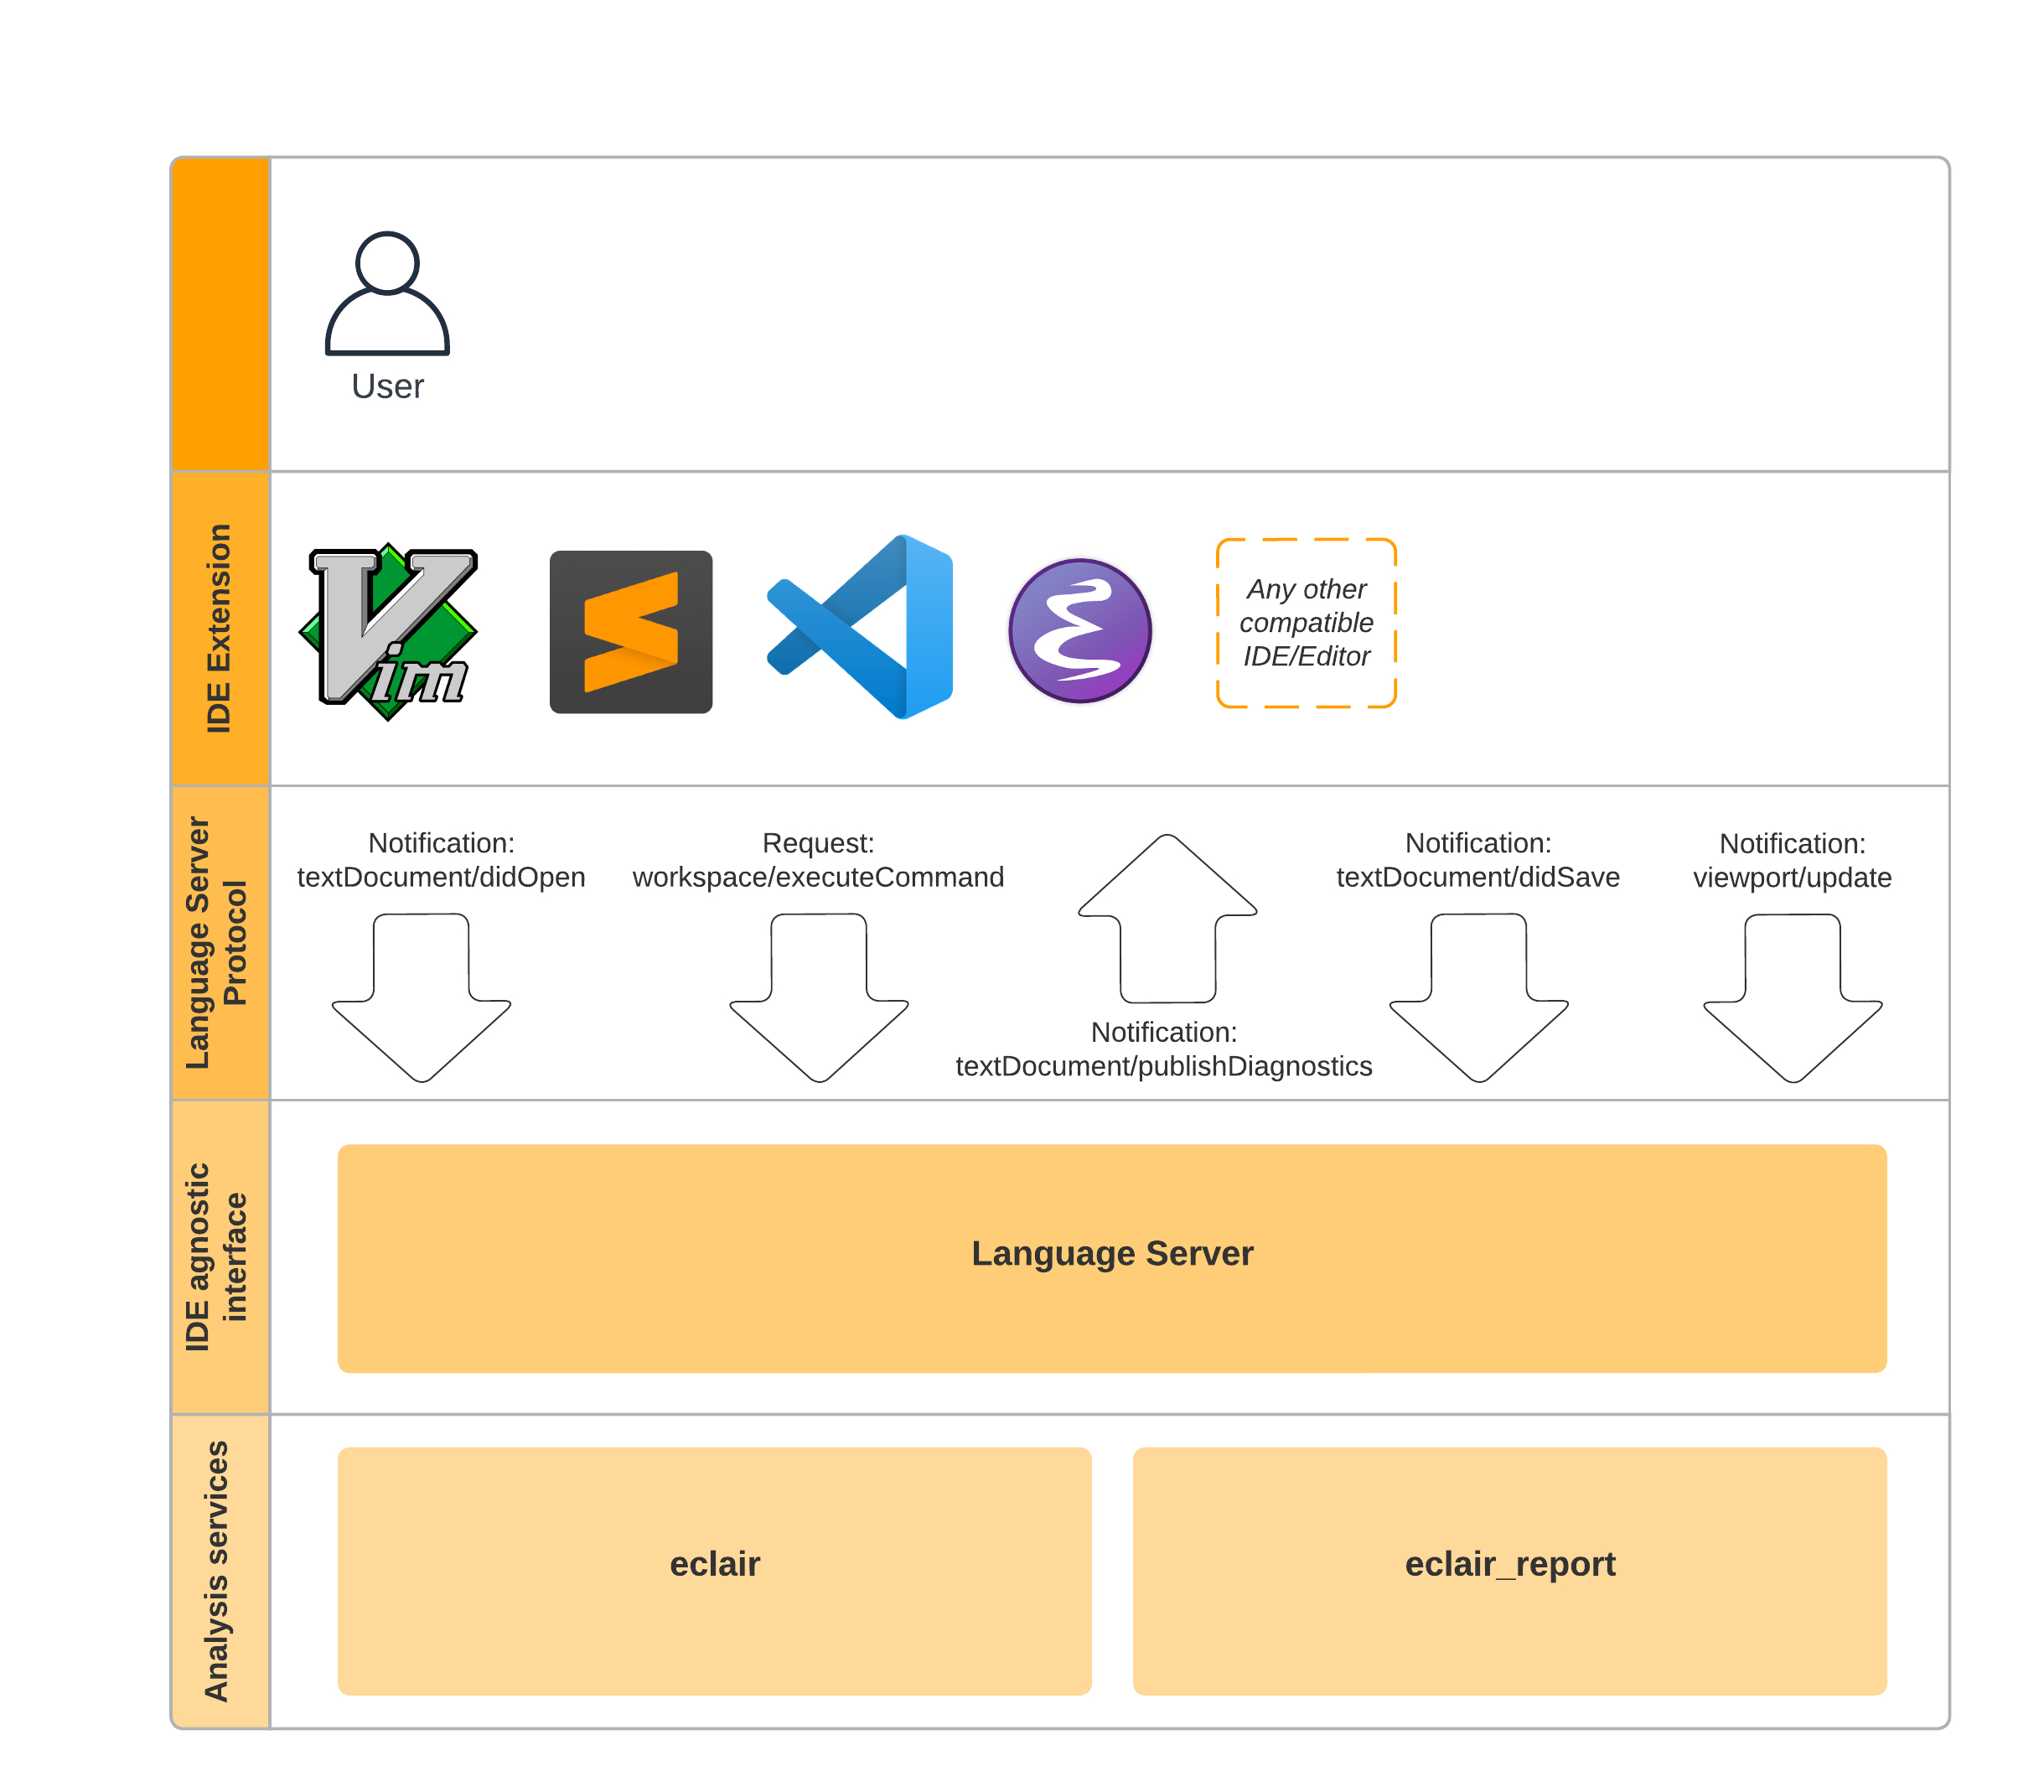
\includegraphics[width=1\textwidth]{Immagini/project_architecture.jpg}
	\caption{Project architecture}
	\label{fig:one}
\end{figure}

The Language Server uses the output received from \emph{eclair\textunderscore	report} to communicate to various IDE extensions, through the LSP, what must be shown to the end user. 

The separation of concerns and the decoupling of the components is at the foundation of this architecture: \emph{eclair\textunderscore	report} is expected to care only about serving the violations to the Language Server, while the \emph{eclair} CLI performs the analysis in an agnostic way regarding how the violations will be served. The only interface the IDE extension has to deal with is the Language Server, which is always the same, independently from the IDE, and hides the complexity of implementing the calls to the analysis services. This way, building new extensions for other IDEs is painless and, with just a few lines of code, it is possible to communicate with the Language Server from the earlier stages of the development. On top of these foundations, extension developers can concentrate on providing the best experience to the end users without worrying about linking the analysis tools to the dishomogeneous IDEs' primitives and APIs.

\section{\emph{eclair}}\label{sec:cap_sec_subsec}
The \emph{eclair} CLI is used to invoke the static analyzer. In order for ECLAIR to work, there must exist an \emph{.ecl} file that specifies:
\begin{itemize}
  \item project-specific configurations;
  \item MISRA rules that should be checked for compliance;
  \item report output format.
\end{itemize}

So the first thing before proceeding with the analysis, is to check for an existing \emph{.ecl} file in the project directory.
\\\\
There are three occasions in which the Language Server invokes the \emph{eclair} CLI:
\begin{itemize}
  \item a new file is opened for the first time;
  \item changes to a file are saved (the user can opt out of this feature);
  \item an analysis is manually triggered.
\end{itemize}

The first two cases are handled automatically whenever the Language Server receives the corresponding notifications, respectively \emph{``textDocument/didOpen''} and \emph{``textDocument/didSave''}. The third case, instead, relies on a \emph{``workspace/executeCommand''} request that is sent from the IDE extension to the Language Server.
\\\\
After performing an analysis, the \emph{eclair} CLI sends its findings to \emph{eclair\textunderscore	report} which in turn saves them into a project internal database, in \emph{.ecd} format. This database will then be used by \emph{eclair\textunderscore	report} to provide the violations.

\begin{figure}[ht]
	\centering
	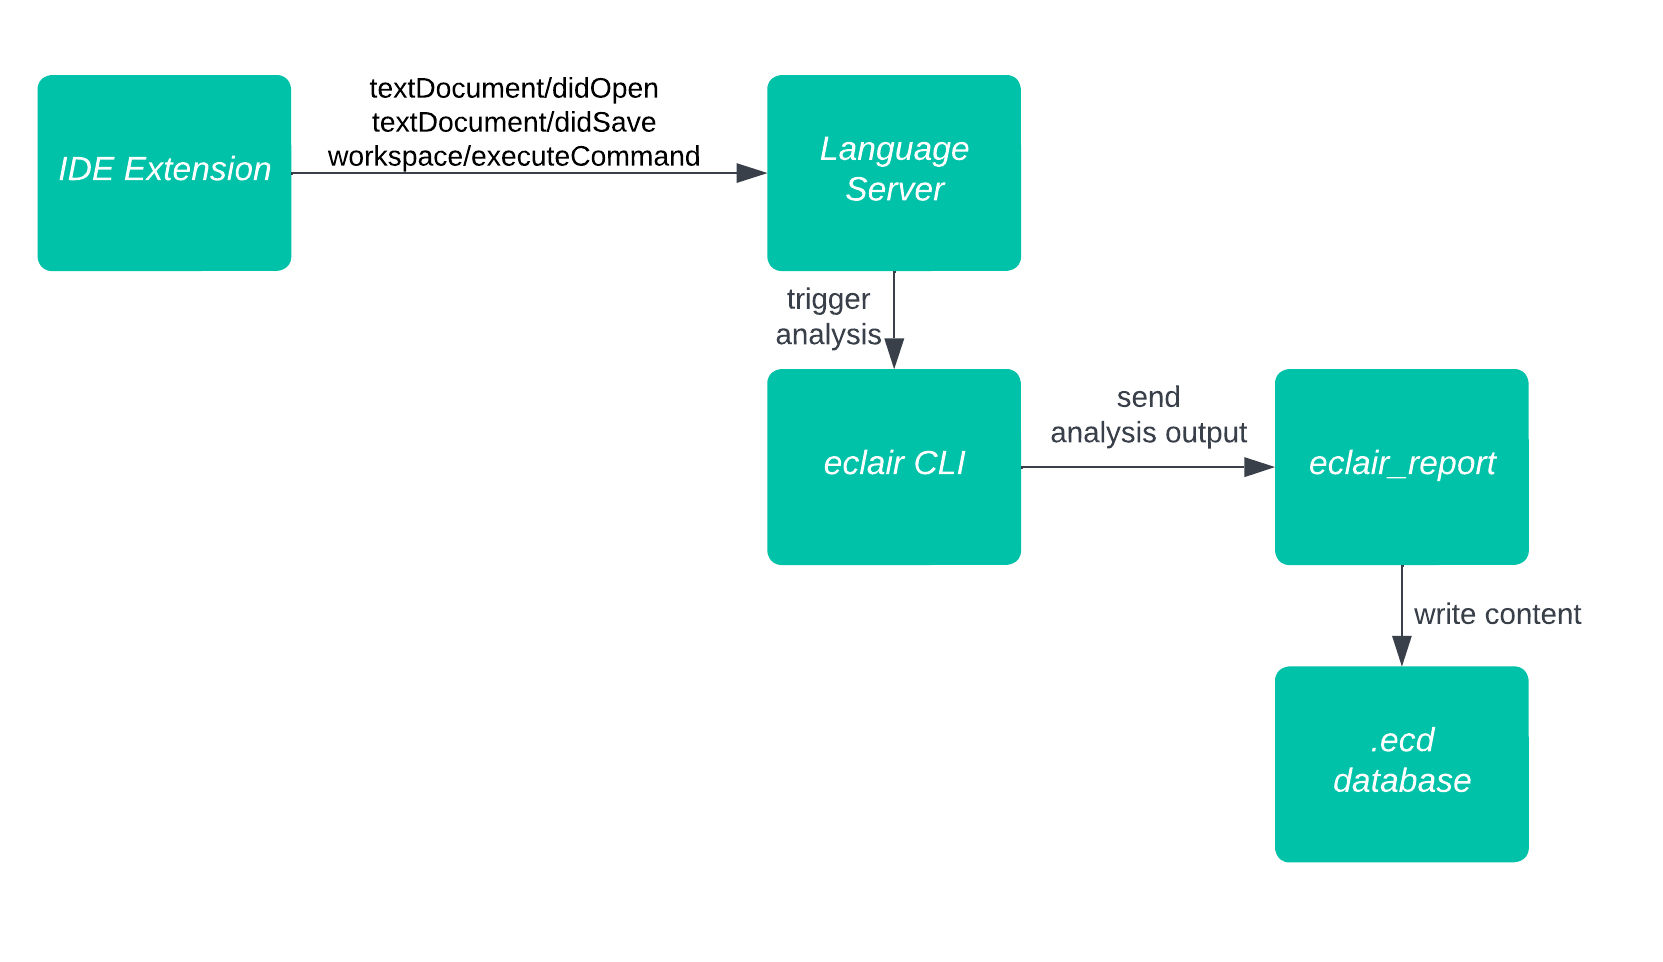
\includegraphics[width=1\textwidth]{Immagini/eclair_analyzer_flow.jpg}
	\caption{Interaction with the \emph{eclair} CLI}
	\label{fig:one}
\end{figure}

\section{\emph{eclair\textunderscore	report}}\label{sec:cap_sec_subsec}
\emph{eclair\textunderscore	report} is already part of the ECLAIR ecosystem: its job is to export ECLAIR analysis findings to different formats (more details about the currently available formats can be found in Chapter~\ref{chapter:starting-point}). 
In the first experiment, described in Chapter~\ref{chapter:the-first-experiment}, the analysis was performed from the beginning whenever the user changed something in the file and violations were returned all at once: unfortunately we noticed that this approach resulted in a slow feedback to the user and sometimes useless analyses were performed. 
\\\\
We decided to use a combination of \emph{eclair} and \emph{eclair\textunderscore	report} to perform the analysis only when necessary and serve its output incrementally. 
The first thing \emph{eclair\textunderscore	report} has to do in our architecture is to save the analysis findings in the project level \emph{.ecd} database. 

Once we had established this, we could build on top of this database features like incrementality and various optimization for the following analyses.
After some reasoning, we decided to proceed with the first, and postpone for now the latter. 

Returning all the violations all at once to the IDE wasn't optimal in particular for huge files: we had to find a new way to navigate them.
We designed a new feature of \emph{eclair\textunderscore	report} that would allow us to interrogate the service and ask incrementally the violations recorded: when interrogated, the tool would be able to receive a top line index and bottom line index and return only the violations in the given range.
Hence, keeping an updated internal state in the Language Server with the current user viewport, we could achieve the incrementality we aimed at. 

\begin{figure}[ht]
	\centering
	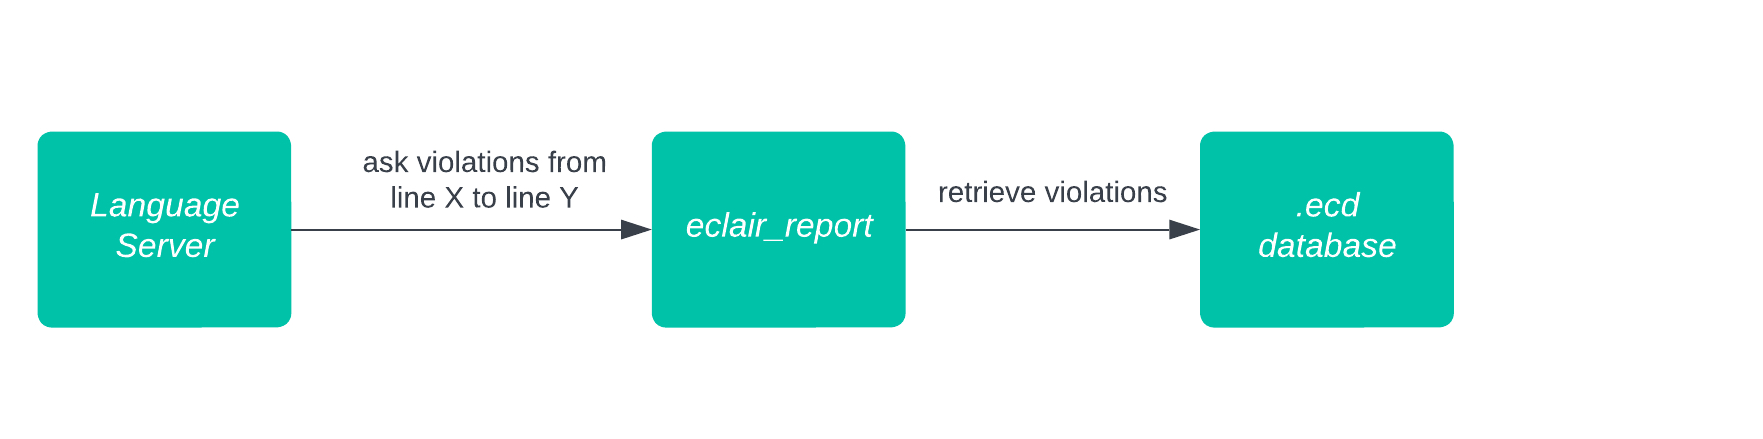
\includegraphics[width=1\textwidth]{Immagini/eclair_report_flow.jpg}
	\caption{Interaction with \emph{eclair\textunderscore	report}}
	\label{fig:one}
\end{figure}

\section{Language Server}\label{sec:language_server_component}
The Language Server is a software written in Typescript, a superset of JavaScript that adds optional static typing to the language, that runs on NodeJS and behaves like a bridge between the ECLAIR ecosystem and the IDE.

In particular, it relies on an implementation of the LSP provided as an NPM library from Microsoft, \lstinline{vscode-languageserver}\footnote{https://www.npmjs.com/package/vscode-languageserver}, and makes the calls to \emph{eclair} and \emph{eclair\textunderscore	report}. 

The Language Server saves an internal representation of the document the user is looking at, incrementally updates it during the editing, and uses it to mark violations.
Every time the user saves the file, opens a new one or manually triggers an analysis a message is sent over to the Language Server, which in turn will trigger an execution by the \emph{eclair} CLI. To avoid useless invocations, the file savings are batched for a defined period of time before making the call asking to perform the analysis.
\begin{lstlisting}[caption={Server side code for viewport synchronization}, label={lst:block_struct}]
type Viewport = {
	filename: string
	topLineIndex: number
	bottomLineIndex: number
}

let viewport: Viewport
const BUFFER = 20

connection.onNotification((method, params) => {
	if (method === ``viewport/update") {
		viewport = params as Viewport

		const uri = ``file://${viewport.filename}"

		connection.sendDiagnostics({
			uri,
			diagnostics: eclairReports.getViolations(workspaceFolder, uri, viewport.topLineIndex - BUFFER, viewport.bottomLineIndex + BUFFER)
		})
	}
})
\end{lstlisting}

\begin{lstlisting}[caption={VSCode extension side code for viewport synchronization}, label={lst:block_struct}]
let lastRecorded = {
	filename: null,
	topLineIndex: null,
	bottomLineIndex: null
}

let timeout: NodeJS.Timeout
Window.onDidChangeTextEditorVisibleRanges(() => {
	if (timeout) {
		clearTimeout(timeout)
	}
	timeout = setTimeout(() => {
		const textEditor = Window.activeTextEditor
		if (textEditor) {
			const visibleRange = textEditor.visibleRanges[0]
			const filename = textEditor.document.fileName
			const topLineIndex = visibleRange.start.line
			const bottomLineIndex = visibleRange.end.line
			if (
				lastRecorded.filename !== filename ||
				lastRecorded.topLineIndex !== topLineIndex ||
				lastRecorded.bottomLineIndex !== bottomLineIndex
			) {
				lastRecorded.filename = filename
				lastRecorded.topLineIndex = topLineIndex
				lastRecorded.bottomLineIndex = bottomLineIndex
				client.sendNotification(``viewport/update", lastRecorded)
			}
		}
	}, 500)
})
\end{lstlisting}
One of the sophistications we had to adopt is the incrementality in the diagnostics: we could not send the violations all at once. However, in order to visualize only the necessary ones, the Language Server must know the file the user is currently looking at and the lines currently in the viewport. 

Unfortunately this feature is not natively offered by the LSP. Thus, inspired from the Text Document Synchronization, we opted for the following approach: whenever the user changes the current active file or viewport, the client retrieves these informations using the IDE's API and uses an LSP notification to send these details to the server, which in turn keeps an internal state. Hence, the Language Server is able to interrogate \emph{eclair\textunderscore	report} and receive only the violations for the file and the lines the user actually needs.

\begin{figure}[ht]
	\centering
	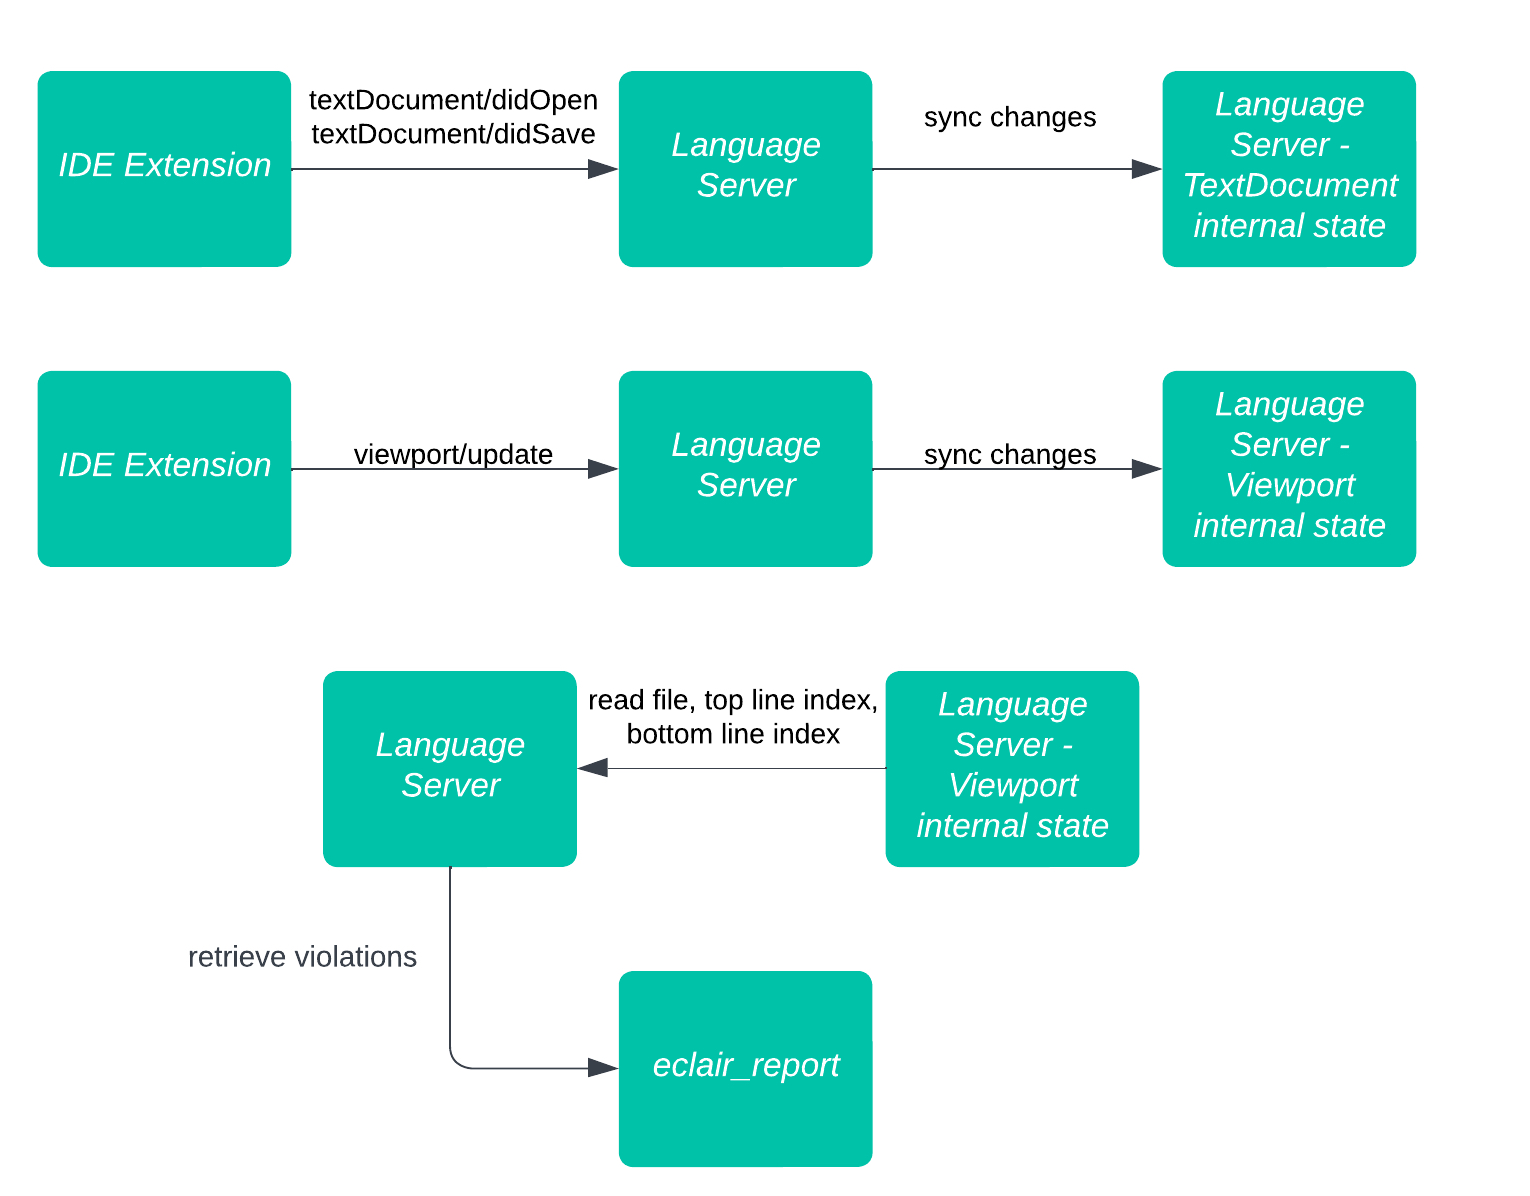
\includegraphics[width=1\textwidth]{Immagini/language_server_flow.jpg}
	\caption{Interactions with the Language Server}
	\label{fig:one}
\end{figure}

\section{VSCode extension}\label{sec:cap_sec_subsec}
The VSCode extension, which in this case exemplifies all the possible IDE plugins/extensions that can be realized on top of this system, has nearly no logic implemented. 
Its main task is the creation of the connection with the Language Server.
\\
In addition to that, some other features, not completely agnostic to the IDE, have been implemented: aside from the viewport synchronization logic, which must retrieve the current viewport using IDE's primitives, already discussed in Section~\ref{sec:language_server_component}, 
we also had to implement a way to manually trigger the analysis and give the user the possibility to opt out from the ``analysis on save'' feature.
Regarding the manually triggered analysis, the Listing~\ref{lst:trigger_analysis_command_code} should give more insights about how we linked the VSCode ``Commands.registerCommand'' API to the ``workspace/executeCommand'' request.
\begin{lstlisting}[caption={VSCode extension triggerAnalysis command}, label={lst:trigger_analysis_command_code}]
Commands.registerCommand(``eclair.triggerAnalysis", () => {
	const uri = Window.activeTextEditor.document.uri
	client.sendRequest(``workspace/executeCommand", {
		command: ``trigger-analysis",
		arguments: [uri.toString()]
	} as ExecuteCommandParams)
})
\end{lstlisting}

On the other hand, the automatic ``analysis on save'' was something we had to think through: a lot of IDEs users have autosaving configurations enabled, so we had to at least make possible to opt out of this feature, given how expensive the analysis is.
We exposed a boolean configuration, \emph{eclair.performAnalysisOnSave}, to switch off the ``analysis on save'' feature and, to fully comply with the LSP approach, we decided that the IDE extension should send over this information with the capabilities in the initialization phase.
In particular, as can be seen on line 14 of Listing~\ref{lst:extension_initialization}, all the content of \emph{Workspace.getConfiguration(``eclair'')} is sent over: if the server is able to use the forwarded settings it will, otherwise they will simply be ignored.

\begin{lstlisting}[caption={VSCode extension initialization}, label={lst:extension_initialization}]
const debugOptions = { execArgv: [``--nolazy", ``--inspect=6011"] }
const serverOptions = {
	run: { module, transport: TransportKind.ipc },
	debug: { module, transport: TransportKind.ipc, options: debugOptions }
}
const clientOptions: LanguageClientOptions = {
	documentSelector: [
		{ scheme: ``file", language: ``c", pattern: ``${folder.uri.fsPath}/**/*" }
	],
	diagnosticCollectionName: ``eclair-language-server",
	workspaceFolder: folder,
	outputChannel: outputChannel,
	progressOnInitialization: true,
	initializationOptions: Workspace.getConfiguration(``eclair")
}
const client = new LanguageClient(``eclair-vscode-client", ``ECLAIR", serverOptions, clientOptions)
client.start()
\end{lstlisting}

Extensibility is at the core of the VSCode plugin and, thanks to the LSP notification based communication, it's simple and intuitive to implement new features, even at different time, on the server and on the client.
In around 200 lines of code, our extension was fully functional and ready to be used as an inspiration to develop other extensions that use the same Language Server.
\begin{figure}[ht]
	\centering
	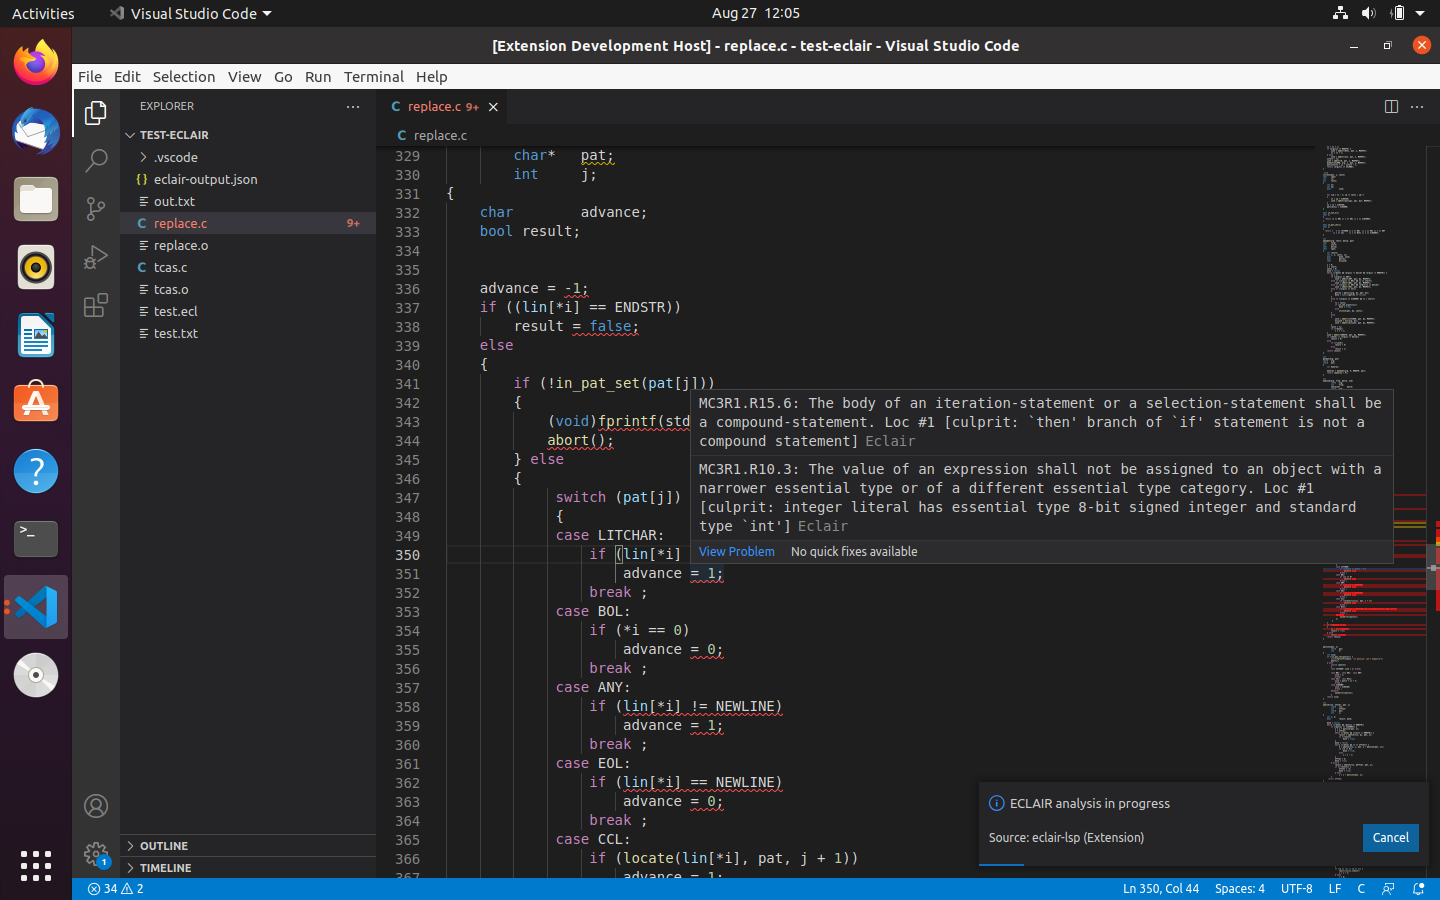
\includegraphics[width=1\textwidth]{Immagini/vscode_extension_screenshot.jpg}
	\caption{A screenshot of the VSCode extension in action}
	\label{fig:one}
\end{figure}